\section{Ergebnisse}
\label{sec:ergebnisse}
Die gemessenen Siedetemperaturen für 11 verschiedene absolute Drücke zwischen \SI{10}{\kilo\pascal} und \SI{100}{\kilo\pascal} sind in Tab. \ref{tab:messwerttabelle} aufgeführt. Die in der rechten Spalte eingetragenen Literaturwerte zu den entsprechenden Drücken entstammen der Literatur \cite{lideCRCHandbookChemistry1994}. An die entnommenen Dampfdrücke zu diversen Temperaturen wurde eine polynomische Funktion fünften Grades angenähert. Das Bestimmtheitsmaß der Funktion beträgt eins. Das bedeutet, dass alle Datenpunkte vom Funktionsgraphen erfasst sind. Durch das Einsetzen der entsprechenden Dampfdrücke konnten damit die exakt passenden Siedetemperaturen zugeordnet werden. Die gefundene Funktion ist außerdem in der Abb. \ref{dia:p/Tmess} abgebildet.
%Tabelle START
\vspace*{-5.5mm}
\renewcommand{\arraystretch}{1.2}
\begin{table}[h!]
	\centering
	\caption{Messwerttabelle und entsprechende Literaturwerte}
	\label{tab:messwerttabelle}
	%\resizebox{12.6cm}{!}{
	\begin{tabular}{|c|c|c|c|}
		\hline
		\textbf{Nr.} &\textbf{p [\si{\kilo\pascal}]}	& \textbf{$\vartheta_{Messung}$ [\si{\degreeCelsius}]} &\textbf{$\vartheta_{Literatur}$ [\si{\degreeCelsius}] \cite{lideCRCHandbookChemistry1994}}	 \\
		\hline
		1& 100 & 81,4 & 82,2 \\
		2& 90 & 78,8 & 79,8 \\
		3& 80 & 76,0 & 77,2\\
		4& 70 & 72,8 & 74,3\\
		5& 60 & 69,2 & 71,1\\
		6& 50 & 65,1 & 67,3\\
		7& 40 & 60,3 & 62,8\\
		8& 30 & 54,3 & 57,1\\
		9& 25 & 50,6 &  53,4\\
		10& 20 & 46,3 & 48,6\\
		11& 10 & 33,7 & 24,1\\
		\hline
	\end{tabular}
	%	}
\end{table}
\FloatBarrier
\vspace*{-2.5mm}
%Tabelle Ende

In der Abb. \ref{dia:p/Tmess} sind die bestimmten Dampfdruckwerte als Funktion der Temperatur aufgetragen. Die Daten können der Tab. \ref{tab:messwerttabelle} entnommen werden.

\begin{figure}[h!]
	\begin{center}
		%\resizebox{0.8\textwidth}{!}{
		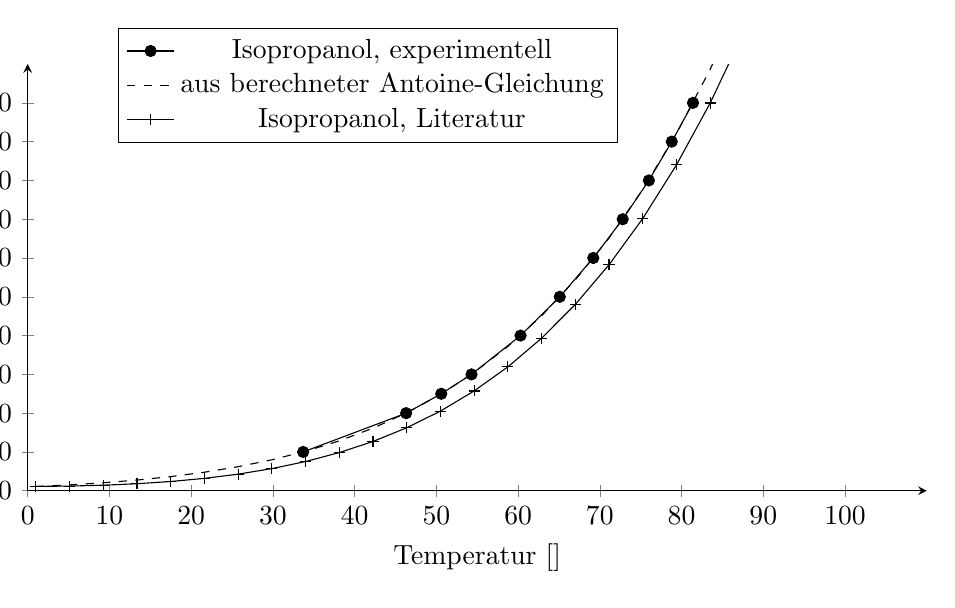
\begin{tikzpicture}[trim axis left, trim axis right]
		\begin{axis}[
		axis lines = left,
		width = 13cm,
		height = 7cm,
		xmin = 0,
		xmax = 110,
		ymin = 0,
		ymax = 110,
		ytick = {0,10,...,100},
		xtick = {0,10,...,100},
		ylabel={Dampfdruck [\si{\kilo\pascal}]},
		y label style={at={(-0.03,0.5)}},
		xlabel={Temperatur [\si{\degreeCelsius}]},
		legend style={at={(0.1,0.95)},anchor=west}
		]
		\addplot[black,mark=*,text mark as node=true,point meta=explicit symbolic,nodes near coords]
		coordinates {(81.4, 100) (78.8, 90) (76, 80) (72.8, 70) (69.2, 60) (65.1, 50) (60.3,40) (54.3,30) (50.6,25) (46.3,20) (33.7,10)};
		
		\addplot +[mark=none, dashed, black, domain=1:100] {8570378.4523 * exp(-3215.05/(x + 201.633))};
		
		\addplot +[mark=+, black, domain=1:100] { 0.00000000425813333333321* x^5 + 0.000000773333333333376*x^4 + 0.0000366666666666613 *x^3 + 0.0032446667 *x^2 +1.11};
		
		\legend{{Isopropanol, experimentell},aus berechneter Antoine-Gleichung,{Isopropanol, Literatur}};
		\end{axis}
		\end{tikzpicture}
		%	}Ventilkennlinie
		\caption{Dampfdruckkurven}
		\label{dia:p/Tmess}
	\end{center}
\end{figure}
\FloatBarrier
\vspace*{-5mm}
Die Abb.\ref{dia:lnp/1/T} stellt die natürlichen Logarithmen der Damppfdrücke in \si{\kilo\pascal} als Funktion über der inversen Temperatur in Kelvin dar. Durch die Schaar der Messpunkte wurde durch lineare Regression im Tabellenkalkulationsprogramm \textsc{Libre-Office Calc} eine Trendlinie berechnet. Die Trendlinie geht auf die Funktionsgleichung (\ref{gl:Regressionsgeradengleichung}) zurück und besitzt ein Bestimmtheitsmaß von 0.99985.
\begin{equation}\label{gl:Regressionsgeradengleichung}
	f(x)=y=-5236.4719735023*x + 19.3850334601
\end{equation}
\begin{figure}[h!]
	\begin{center}
		%\resizebox{0.8\textwidth}{!}{
		\begin{tikzpicture}[trim axis left, trim axis right]
		\begin{axis}[
		axis lines = left,
		width = 13cm,
		height = 7cm,
		xmin = 0.0028,
		xmax = 0.00337,
		ymin = 2.2,
		ymax = 5,
		ytick = {2.2,2.6,3,3.4,3.8,4.2,4.6},
		xtick = {0.0028,0.0029,0.003,0.0031,0.0032,0.0033},
		ylabel={ln(p) [\si{\kilo\pascal}]},
		y label style={at={(-0.03,0.5)}},
		xlabel={1/T [\si{\kelvin}]},
		legend style={at={(0.1,0.95)},anchor=west}
		]
			\addplot table {ln(p)ueber1durchT.dat};
		
			\addplot +[mark=none, dashed, black, domain=0.0027:0.00338] {-5236.4719735023*x + 19.3850334601};
		\legend{T={Isopropanol, experimentell},Trendline nach Gleichung  (\ref{gl:Regressionsgeradengleichung}),T=\SI{37,0}{\celsius}};
		\end{axis}
		\end{tikzpicture}
		%	}Ventilkennlinie
		\caption{Natürlicher Logarithmus des Dampfdruckes über der inversen Temperatur}
		\label{dia:lnp/1/T}
	\end{center}
\end{figure}
\FloatBarrier
\vspace*{-5mm}

\subsection{Berechnung der molaren Verdampfungsenthalpie}\label{sec:berechnungMolareVerdEnthalpie}
Die Berechnungs der molaren Verdampfungsenthalpie $\Delta_{LV}H_m$ baut auf der Clausius-Clapeyron-Gleichung auf. Es müssten folgende Annahmen getroffen werden.
\begin{itemize}
	\item Das molare Volumen der flüssigen Phase wird gegenüber dem molaren Volumen der Gasphase vernachlässigt.
	\item Für den Dampf wird ideales Gasverhalten angenommen.
\end{itemize}
Daraus ergibt sich dann die Gleichung (\ref{gl:verdampfungsenthalpie}). Der linke Teil der Gleichung beschreibt dabei den Anstieg der zuvor ermittelten Regressionsgerade. Die Annahme idealen Gasverhaltens erlaubt auch die Verwendung der idealen Gaskonstante $R$.	\cite{molareVerdampfungsenthalpie}

\begin{flalign}\label{gl:verdampfungsenthalpie}
	\frac{d(\ln(p))}{d(1/T)}&=-\frac{\Delta_{LV}H_m}{R}\\
	\SI{-5236,472}{\kelvin}&=-\frac{\Delta_{LV}H_m}{\SI{8,314}{\joule\per\mole\per\kelvin}}\\
	\Delta_{LV}H_m&=\underline{\underline{\SI{43,536}{\kilo\joule\per\mole}}}
\end{flalign}

\subsection{Berechnung der Dampfdruckkurve aus den ermittelten \textit{ANTOINE}-Konstanten}\label{sec:berechnungDampfdruckkurveausKonstanten}

Die ermittelten \textit{ANTOINE}-Konstanten derl Tab.\ref{tab:AntoineKonstanten} werden in die \textit{ANTOINE}\-Gleichung eingetragen. Dieser Schritt kann anhand der Gl.(\ref{gl:antoineEingesetzt}) nachvollzogen werden.
\begin{flalign}\label{gl:antoineEingesetzt}
	\lg(p)&=A-\frac{B}{C+\vartheta \,[\si{\degreeCelsius}]}\\
	\lg(p)&=6,933-\frac{1396,28}{201,633+\vartheta\, [\si{\degreeCelsius}]}\\
	p&=8570378,452304*e^{\frac{-3215,0535}{T+201,633}}
\end{flalign}
Die so erhaltene Dampfdruckkurve ist in die Abb.\ref{dia:p/Tmess} eingetragen. 